\def\year{2016}
\documentclass[letterpaper]{article}
\usepackage{aaai}
\usepackage{times}
\usepackage{helvet}
\usepackage{courier}
\setlength{\pdfpagewidth}{8.5in}
\setlength{\pdfpageheight}{11in}

\usepackage{graphicx}
\usepackage{algorithm}
\usepackage[noend]{algpseudocode}
\usepackage{amsmath}
\usepackage{amssymb}
\usepackage{amsthm}
\usepackage{etoolbox}
\usepackage{color}
\usepackage{changepage}
\usepackage{csquotes}
\usepackage{tabularx,booktabs,multirow}
\usepackage{longtable}

\pdfinfo{
/Title (Learning Constraints and Optimization Criteria)
/Author (Samuel Kolb)}
\setcounter{secnumdepth}{1}  

\graphicspath{{Graphics/}{}}

\newcommand{\sym}[1]{\ensuremath{\mathcal{#1}}}
\newcommand{\svm}{SVM$^{rank}$}

\newtheorem{question}{Question}
\theoremstyle{definition}
\newtheorem{example}{Example}

\newcommand{\sam}[1]{{\color{red}(#1)}}
\newcommand{\abs}[1]{\left|#1\right|}

\setlength{\tabcolsep}{6pt}

\title{Learning Constraints and Optimization Criteria}
\author{
  Samuel Kolb\\
  KU Leuven, Leuven, Belgium\\
  samuel.kolb@cs.kuleuven.be
}

\begin{document}

\maketitle

\begin{abstract}
While there exist several approaches in the constraint programming community to learn a constraint theory, few of them have considered the learning of constraint optimization problems.
To alleviate this situation, we introduce an initial approach to learning first-order weighted MAX-SAT theories. 
It employs inductive logic programming techniques to learn a set of first-order clauses and then uses preference learning techniques to learn the weights of the clauses.
In order to learn these weighted clauses, the clausal optimization system uses examples of possible worlds and a set of preferences that state which examples are preferred over other ones.
The technique is also empirically evaluated on a number of examples.
These experiments show that the system is capable of learning clauses and weights that accurately capture underlying models.
\end{abstract}

% -------------------------------------------------
% Introduction
% -------------------------------------------------

% \begin{itemize}
%   \item \sam{Why interesting, connection to Campignotto, Domingos, Kok, Why preferences useful?}
%   \item \sam{Real tasks with preferences? Small scale evaluation}
%   \item \sam{Lot of background knowledge assumed (vs. constraint programming, probabilistic programming, demo model and need for learning!)}
% \end{itemize}

\section{Introduction}
An important class of declarative models is concerned with (discrete) constrained optimization problems.
These combine constraint satisfaction problems with an optimization function that specifies which solutions are optimal.
While these models are powerful and elegant, they are often also hard to obtain, certainly for non-experts \cite{Wallace:PrinciplesCP}.
This has motivated several researchers to investigate whether such models can be learned. 

Constraint learning is the task of discovering constraints from data.
This task has been addressed in constraint programming (e.g. \cite{Beldiceanu:ModelSeeker,bessiere2013constraint}) and inductive logic programming (e.g. \cite{DeRaedt:ClausalDiscovery}).
Recent efforts \cite{Lallouet:LearningCP} have attempted to combine these two fields.
Furthermore, \cite{campigotto2011active} have learned propositional weighted MAX-SAT theories from examples.

We use weighted first-order logical theories to represent constrained optimization problems (as illustrated in example~1).
The weights capture the optimization function, and (first-order) weighted MAX-SAT can be used to determine the \emph{best} solutions.
Furthermore, we learn such models by combining inductive logic programming (ILP) principles (such as clausal discovery \cite{DeRaedt:ClausalDiscovery}) with preference learning.
We use ILP to learn the clausal theories from interpretations, and preference learning to determine the weights.
Therefore, users provide examples of possible worlds and a set of preferences that specify which examples are preferred over other ones.
This setting extends traditional constraint learning and ILP approaches with the ability to learn soft constraints and integrates constraint satisfaction and optimization.
It also extends the propositional approach of \cite{campigotto2011active} as first-order theories are learned and preferences are used rather than examples with target values.
Preferences are useful in situations where the score of an example is hard to quantify (e.g. comparing songs or designs) and it is often easier for humans to provide preferences over few examples at a time than absolute scores.

Weighted first-order MAX-SAT problems relate to Markov Logic networks (MLN), as MAP inference in MLNs can be used to query for the most likely state.
Therefore, work in statistical relational learning (SRL) on learning the structure of MLNs or other SRL models \cite{kok2005learning} is also relevant.
However, our work differs from the SRL and MLN approaches in that one learns from preferences rather than from examples.

% We use preferences for learning as it is often easier for humans to provide preferences over few examples at a time than absolute scores.
% This makes them useful in interactive settings and in situations where an examples absolute score is hard to quantify.

% One of the main advantages of using preferences for learning is that preferences are often easier to provide for humans and only consider few examples at a time.
% Consequently, they are useful in interactive settings and in situations where an examples absolute score is hard to quantify.


This paper is organized as follows.
Section~2 reviews background and related work.
We introduce the formalism and the setting in Section~3, the algorithm and the clausal optimization system in Section~4, and in Section~5 we report on some experiments.
Finally, Section~6 concludes this paper.

% -------------------------------------------------
% Background
% -------------------------------------------------

\section{Background}
In this section we provide a brief overview of the important concepts and relevant literature.

\paragraph{Clauses}
We use (function free) first-order clauses; which we now introduce.
An atom $P(t_1, t_2, ..., t_n)$ consists of a predicate symbol~$P$ that is applied to $n$ terms~$t_i$.
Terms are either constants or variables.
In this paper predicates and constants will be written in uppercase ($\mathit{John}$) and variables in lowercase ($\mathit{x}$).
A literal can be an atom~$a$ (positive literal) or a negated atom~$\lnot a$ (negative literal).
Clauses are disjunctions of literals $l_1 \lor l_2 \lor ... \lor l_k$ and are assumed to be universally quantified.
A clause can be expressed using a body and a head $\mathit{head} \leftarrow \mathit{body}$.
Hereby, positive literals are grouped in the head and negative literals are grouped in the body.
Sometimes clauses are also written as sets of literals $\{l_1, l_2, ..., l_k\}$.

Atoms are grounded if they contain no variables.
A Herbrand interpretation is a set of ground atoms.
All atoms in the interpretation are assumed to be true and all other possible ground atoms are assumed to be false.
$\sym{I} \models c$ is used to denote that interpretation \sym{I} satisfies the clause $c$.

\paragraph{Optimization}
The Boolean Satisfiability problem (SAT) is the problem of determining whether a propositional formula can be satisfied.
Formulas can be rewritten into Conjunctive Normal Form (CNF), which consists of a conjunction of clauses (disjunctions).
An extension of this problem is the Maximum Satisfiability Problem (MAX-SAT), which is an optimization problem and attempts to maximize the number of satisfied clauses.
By assigning positive integer weights to clauses and maximizing the sum of the weights of satisfied clauses, one obtains the weighted MAX-SAT problem.

In related work \cite{campigotto2011active} weighted MAX-SAT problems are induced by learning propositional clauses and weights using examples and absolute scores.
The representation we use is an extension of weighted MAX-SAT to first-order logic.
We also learn this model using preferences over sets of examples (possible worlds), rather than assigning target values to examples.

\paragraph{Constraint Learning}
The goal of constraint learning is to automatically identify constraints in one or multiple examples.
This task is difficult because the search space of constraints is typically very large and, unlike in typical machine learning problems, there are usually only few examples to learn from.

There are different approaches to accomplishing this task.
The problem of having little examples can be alleviated by interactively generating data.
Both the systems Conacq2 \cite{bessiere2007query} en QuAcq \cite{bessiere2013constraint} generate (partial) examples and query the user about their validity.

ModelSeeker \cite{Beldiceanu:ModelSeeker} structures the problem variables in different ways.
A large catalog of global constraints is used to find constraints that hold within this structure.
This approach allows for constraint learning from a few examples.

As mentioned earlier, the research of \cite{Lallouet:LearningCP} uses ILP techniques to learn constraints.
They explore the search space of constraints in a bidirectional manner, primarily using negative examples.

% -------------------------------------------------
% Problem Statement
% -------------------------------------------------

\section{Problem Statement}
\label{sec:problem}
We want to learn constraints and optimization criteria based on positive examples and user preferences.
Since our aim is to simplify the process of generating formal representations, any input should be reasonably easy for a user to provide.

In order to apply ILP techniques for constraint learning, we will use first-order logical clauses as constraints.

\paragraph*{Clause Learning}
\emph{Given a set of examples and a threshold $t$, find maximally specific clauses that are satisfied by at least $t$ of the given examples.}
\\\\
Examples are Herbrand interpretations.
They consist of a set of constants, the domain, and all ground atoms over these constants that are true.
The learned clauses are domain-independent hard or soft constraints and contain only variables.
\\\\
Our goal is to learn optimization criteria, weighted soft constraints, based on examples (interpretations) and user preferences.
A (pairwise) preference $e_1 \succ e_2$ describes a relative order over examples $e_1$ and~$e_2$, stating that $e_1$ is preferred over~$e_2$.
Preferences only consider two examples at a time and are usually easier to provide than absolute scores.
The soft constraints consist of clauses~(\sym{C}) that are satisfied by some but not all of the examples.
They can be identified using a system that implements the constraint learning task.
Weighted clauses~($\sym{W}_{\sym{C}}$) are tuples $\mathbb{R} \times \sym{C}$ that can be used to calculate a score for any example $e$:
\begin{eqnarray}
  \label{eqn:score}
  score_{\sym{W}_{\sym{C}}}(e) = \sum\limits_{(\mathit{w}, \mathit{c}) \in \sym{W}_{\sym{C}}} \mathit{w} \cdot \mathbf{1}_{e \models c}
\end{eqnarray}
An interpretation~$e_{opt}$ is an optimal solution with respect to~$\sym{W}_{\sym{C}}$ if $score_{\sym{W}_{\sym{C}}}(e_{opt})$ is maximal.

\begin{example}[Moving city]
  \label{ex:moving}
  Consider the scenario of moving to a new city and choosing areas for housing, work and school.
  The choices are captured by the predicates $\mathit{LiveIn}$, $\mathit{WorkIn}$ and $\mathit{SchoolIn}$.
  Additionally, the predicates $\mathit{Cheap}$ and $\mathit{LowCrime}$ are used to designate cheap and low crime areas, respectively.

  Assume the following set of weighted clauses~\sym{M} describes the optimization problem to solve:
  \begin{flalign*}
    (w_1, c_1) &= (0.50, \mathit{LowCrime}(a) \leftarrow \mathit{LiveIn}(a)) \\
    (w_2, c_2) &= (0.25, \mathit{SchoolIn}(a) \leftarrow \mathit{WorkIn}(a)) \\
    (w_3, c_3) &= (1.00, \mathit{LowCrime}(a) \leftarrow \mathit{SchoolIn}(a)) \\
    (w_4, c_4) &= (-1.00, \mathit{false} \leftarrow \mathit{LiveIn}(a) \land \mathit{Cheap}(a))
  \end{flalign*}
  Let examples $e_1$, $e_2$ and~$e_3$ be Herbrand interpretations that reason over the same city, using the same constants (areas) $A_1$, $A_2$ and $A_3$.
  Consider the set~\sym{S} of shared ground atoms $\{\mathit{Cheap}(A_1)$, $\mathit{Cheap}(A_3)$, $\mathit{LowCrime}(A_1)$, $\mathit{LowCrime}(A_2)\}$ and define the examples as:
  \begin{flalign*}
    &e_1 = \{\mathit{LiveIn}(A_1), \mathit{WorkIn}(A_2), \mathit{SchoolIn(A_2)}\} \cup \sym{S} \\
    &e_2 = \{\mathit{LiveIn}(A_2), \mathit{WorkIn}(A_2), \mathit{SchoolIn(A_3)}\} \cup \sym{S}\\
    &e_3 = \{\mathit{LiveIn}(A_2), \mathit{WorkIn}(A_2), \mathit{SchoolIn(A_1)}\} \cup \sym{S}.
  \end{flalign*}

  The score of an example can be calculated using~(\ref{eqn:score}).
  Example~$e_1$ is covered by clauses $c_1$, $c_2$ and~$c_3$, therefore, $score_{\sym{M}}(e_1) = 0.5 + 0.25 + 1 + 0 = 1.75$.
  Analogously we can compute $score_{\sym{M}}(e_2) = -1$ and $score_{\sym{M}}(e_3) = 0$.
  Using $score_{\sym{M}}$, the following preferences can be generated: $e_1 \succ e_2$, $e_1 \succ e_3$ and $e_2 \succ e_3$.
\end{example}

The aim of our research is to learn weighted clauses such that the order imposed by these optimization criteria maximally corresponds with the given preference information.

\paragraph*{Clausal Optimization}
\emph{Given examples~\sym{E}, preferences~\sym{P} and threshold~$t$, learn clauses~\sym{C} that cover at least $t$ examples and find weights~$\sym{W}_{\sym{C}}$ that maximize:
\begin{flalign*}\abs{\{e_1 \succ e_2 \in \sym{P} | score_{\sym{W}_{\sym{C}}}(e_1) > score_{\sym{W}_{\sym{C}}(e_2, })\}}.\end{flalign*}}

% -------------------------------------------------
% Approach
% -------------------------------------------------

\section{Approach}
We use a two-step approach to learn weighted first-order clauses.
First, clause learning is used to find soft constraints in the given examples.
Then, user-provided preference information is used to learn weights for these constraints.

% \begin{example}
%   \label{ex:moving-input}
%   Consider the moving problem (example~\ref{ex:moving-input}).
%   A model could, for example, use a type \textit{Area} and predicate definitions low\_crime(\textit{Area}), cheap(\textit{Area}), school\_in(\textit{Area}), work\_in(\textit{Area}) and live\_in(\textit{Area}).
%   Examples would then specify various areas $A_i$ and describe the conditions (e.g. cheap($A_1$), low\_crime($A_2$)) as well as the users choices (e.g. school\_in($A_2$), work\_in($A_2$), live\_in($A_1$)).
%   % Imagine a problem that describes humans with a type \textit{human} and predicates human(\textit{human}), male(\textit{human}) and female(\textit{human}).
%   % An example could contain the constants S and A, both of type \textit{human}, and the relations: human(S), human(A), male(S), female(A).
%   % Clauses to be learned would be: human(x) $\leftarrow$ male(x), human(x) $\leftarrow$ female(x),  female(x) $\lor$ male(x) $\leftarrow$ human(x) and \textit{false} $\leftarrow$ female(x) $\land$ male(x).
% \end{example}

\begin{algorithm}
  \caption{The clausal discovery algorithm}
  \label{alg:cd}

  \begin{algorithmic}
  \State Given: Examples \sym{E} and threshold $t$
  \State $\sym{Q} \gets \{\square\}$, $\sym{T} \gets \{\}$
  \While{$\abs{\sym{Q}} > 0$}
    \State $c \gets next(\sym{Q})$
    \If{$\abs{\{e \in \sym{E} | e \models c\}} \geq t$}
      \If{$\sym{T} \not\models c$}
        \State $\sym{T} = \sym{T} \cup c$
      \EndIf
    \Else
      \State $\sym{Q} \gets \sym{Q} \cup \rho(c)$
    \EndIf
  \EndWhile
  \State $\sym{T} \gets prune(\sym{T})$
  \State \Return \sym{T}
  \end{algorithmic}
\end{algorithm}

\subsection{Clause Learning}
The clause learning system is based on clausal discovery \cite{DeRaedt:ClausalDiscovery}.
Algorithm~\ref{alg:cd} illustrates how clausal discovery works on a high level.
To compute if a clause~$c$ covers enough examples, the number of examples~$e$ is counted for which $e \models c$ (i.e. $c$ is true in the example~$e$ or $c$ covers $e$).
In order to remove redundant clauses a new clause~$c$ is only added to the result set $\sym{T}$ if $\sym{T} \not\models c$ (i.e. $c$ is not logically entailed by \sym{T}).
Both $e \models c$ and $\sym{T} \not\models c$ are computed by the IDP knowledge base system \cite{de2013prototype,wittocx2008idp}.
The algorithm can find both soft constraints ($t < \abs{\sym{E}}$) or hard constraints ($t = \abs{\sym{E}}$).

Starting with the empty clause ($\square$), clauses are refined until they cover enough examples.
If a clause covers enough examples it is added to the result set, unless it is entailed by clauses already in the result set.
In the refinement step, a clause $c = \{l_1, l_2, ..., l_k\}$ is extended (refined) by adding a new literal $l$.
The new clause, $c' = c \cup \{l\}$ is more general than $c$ ($c' \models c$) and potentially covers more examples.
By adding just one literal the refinement operator $\rho$ generates the set of clauses that are minimally more general.
In order to do this efficiently, our implementation uses a pre-calculated list of atoms, given a maximal number of variables that can occur within a clause.
Within the body and head of a clause, atoms may only be added in a specific order to avoid generating redundant clauses.

A few additional measures are used to make the implementation more efficient.
Most importantly, there are two syntactic restrictions on the form of the clauses.
Clauses must be connected (i.e. new atoms must always contain a variable that has already occurred) and range-restricted (i.e. no new variables may be introduced in the head of the clause).
Moreover, Object Identity is used to specify that variables with different names must denote different objects.
Therefore, a clause~$c$ with variables \sym{V} is extended to the clause~$c_{OI}$ by adding literals $x_i \neq x_j$, for $x_i, x_j \in \sym{V}, i \neq j$.
Finally, the implementation natively supports typed constants and predicates, symmetric predicates (i.e. predicates where the order of terms does not matter) and background knowledge.
A predicate can be marked as \emph{calculated} in which case it is defined in the background knowledge, rather than being provided in the examples. 

\subsection{Clausal Optimization}
In order to find weighted soft constraints, the clause learning system is used with a low threshold to learn (soft) clauses~\sym{C}.
The examples are then translated to Boolean feature vectors of length $\abs{\sym{C}}$ by introducing a feature for every clause~$c_i \in \sym{C}$.
For an example~$e$, the value of its feature vector $\mathbf{v}_e$ for clause~$c_i$ is calculated as $\mathbf{v}_e(i) = \mathbf{1}_{e \models c_i}$.
Next, a linear function $f(\mathbf{v})=\sum_i w_i \cdot \mathbf{v}(i)$ is learned that assigns weights~$w_i$ to clauses~$c_i$, based on the user-provided preferences.
The scoring function~$f$ agrees with a preference $e_1 \succ e_2$ if $f(\mathbf{v}_{e_1}) > f(\mathbf{v}_{e_2})$ and corresponds to the scoring function (\ref{eqn:score}).

\begin{example}
  \label{ex:features}
  Consider examples~$e_1, e_2, e_3$, preferences $e_1 \succ e_2, e_2 \succ e_3$ and clauses $c_1, c_2, c_3$, whereby clauses cover examples according to Table~\ref{tbl:cover_examples}.
  The function $f(\mathbf{v}) = (1, 0, -2) \cdot \mathbf{v}$ assigns scores $f(\mathbf{v_{e_1}}) = 1$, $f(\mathbf{v_{e_2}}) = 0$ and $f(\mathbf{v_{e_3}}) = -1$ and perfectly models the given preferences since $f(\mathbf{v_{e_1}}) > f(\mathbf{v_{e_2}})$ and $f(\mathbf{v_{e_2}}) > f(\mathbf{v_{e_3}})$.
  This score has no value in the absolute sense, it can only be used to compare between examples.
  In this example clause~$c_1$ represents a desirable property and clause~$c_3$ represents an undesirable property.

  \begin{table}
  \caption{Clause coverage}
  \label{tbl:cover_examples}
  \begin{tabularx}{\linewidth}{c|l|X}
    \textbf{Example} & \textbf{Covered by} & \textbf{Feature vector}\\
    \toprule
    $e_1$             & $c_1$               & $\mathbf{v}_{e_1} = (1, 0, 0)$ \\
    $e_2$             & $c_2$               & $\mathbf{v}_{e_2} = (0, 1, 0)$ \\
    $e_3$             & $c_1$, $c_2$, $c_3$ & $\mathbf{v}_{e_3} = (1, 1, 1)$ \\
  \end{tabularx}
  \end{table}
\end{example}

\svm{} \cite{joachims2006training} was chosen to find the scoring function since it uses a linear model and offers a robust and efficient implementation.
The weights that it assigns to the features can be used directly as weights for the clauses.
Other linear ranking systems such as Coordinate Ascent \cite{metzler2007linear} could also be used.

\subsection{Optimal Solution}
Typical MAX-SAT solvers use propositional clauses and only allow for positive weights.
However, the first-order logic solver IDP can solve our optimization task as it supports inductive definitions, aggregates and minimization.
The only limitation is that the current version is restricted to integer values and does not support rational numbers.
Therefore, the weights of the clauses are divided by the smallest absolute weight, multiplied by a constant and rounded to the closest integer.

In order to model the optimization problem in IDP, every clause $c_i$ with variables $v_1, ..., v_n$ is represented by a number $i$. For every clause a predicate $T(i)$ is added to capture the truth value of the clause.
A function $\mathit{Cost}(i)$ specifies the cost of not satisfying the clause, which is equal to the weight of the clause.
\begin{flalign*}
  &T(i) \Leftrightarrow \forall v_1, ..., v_n : c_i. \\
  &Cost(i) = w_i.
\end{flalign*}

Using $T$ and $\mathit{Tost}$, a function $\mathit{Actual}(i) = \mathbf{1}_{\lnot T(i)} \cdot \mathit{Cost}(i)$ is then defined inductively.
This function is used in the optimization criterion $\sum_i Actual(i)$ which should be minimized. % , which will allow IDP to search for an optimal solution.

% -------------------------------------------------
% Evaluation
% -------------------------------------------------

\section{Evaluation}
In our experiments we aim to measure the accuracy and efficiency of the learning systems for constraints and optimization criteria.
Non-deterministic experiments (e.g. measuring execution times or accuracy of clausal optimization) were repeated eight times and their result were averaged.
Some problems and experiments are only described briefly or summarized, for more details we refer to \cite{kolb2015thesis}\footnote{Available online at https://github.com/samuelkolb/thesis}.

First, experiments concerning the accuracy and efficiency of the constraint learning implementation are discussed.
Thereafter, we discuss the evaluation of the accuracy of the clausal optimization system\footnote{The system (v1.0) used to perform all experiments is available online at https://github.com/samuelkolb/clausal-discovery/releases}.

\subsection{Clause Learning}
We used four problems to evaluate constraint learning:
\begin{description}
\item[Map Coloring] Countries are assigned colors and neighboring countries may not have the same color.
Two examples, each containing three correctly colored countries, are given.
\item[Sudoku] A single, solved $4 \times 4$ sudoku is given as an example for this problem.
\item[Elevator] This problem uses three predicates $\mathit{Inside}$, $\mathit{Crowded}$ and $\mathit{Panic}$, with $\mathit{Crowded}$ being a calculated predicate.
It is defined by background knowledge to be true for all elevators with three or more people inside.
Out of the three examples provided for this problem, two satisfy the target soft constraint:
\begin{flalign*}
  &\mathit{Panic}(p)~\leftarrow~\mathit{Crowded}(e)~\land~\mathit{Inside(p, e)}.
\end{flalign*}
\item[Co-housing] The co-housing problem also uses background knowledge to specify one of its predicates ($\mathit{Cheap}$) and to impose some additional constraints.
Five examples are provided, which all adhere to the following four constraints on the housing choices of two friends:
\begin{enumerate}
  \item If the two friends do not live in the same area, they work in the same area.
  \item If a person does not work and live in the same area, that person needs a car.
  \item A person who lives in a cheap area has a car.
  \item If the two friends live together, they live in an expensive area.
\end{enumerate}
\end{description}
The clausal discovery implementation is used to learn soft constraints for the elevator problem ($t = 1$) and hard constraints for the other problems.

\begin{question}[Accuracy]
  Are the essential constraints discovered and what influence do different parameters have on the accuracy?
\end{question}
For all problems the essential constraints are found.
Often additional constraints were found that describe some structure in the problems.
For example, for the map coloring problem one of the learned constraints states that countries are never their own neighbor.
These kind of constraints may help a constraint solver to work more efficiently.

The learning process is parameterized by the maximal number of variables and literals allowed per clause.
If these limits are too large, constraints are found that over-fit the training data.
These constraints are too specific and will exclude valid solutions that are not in the training set.
Over-fitting can be addressed by removing invalid constraints (manually or automatically) and providing more (or larger) training examples.
On the other hand, if the chosen limits are too small, the necessary constraints will not be found.
Under-fitting can be detected using negative examples.

\begin{table}
  \caption{Execution times for learning constraints}
  \begin{tabularx}{\linewidth}{r|X}

\textbf{Problem}    & \textbf{Average time (s)} \\ % & \textbf{Time (baseline)}  
\toprule
Map Coloring        & 1.581   ($\pm$ 0.117)     \\ % & 1.000                     
Sudoku              & 4.787   ($\pm$ 0.062)     \\ % & 1.000                     
Elevator            & 3.182   ($\pm$ 0.073)     \\ % & 1.000                     
Co-housing          & 25.903  ($\pm$ 0.446)      % & 1.000                     
% \midrule
% Range             & Map coloring        & 4.629   ($\pm$ 0.199)     \\ % & 2.928                     
% restriction       & Sudoku              & 16.118  ($\pm$ 0.154)     \\ % & 3.367                     
%                   & Elevator            & 40.453  ($\pm$ 0.319)     \\ % & 12.713                    
%                   & Co-housing          & 207.768 ($\pm$ 0.330)     \\ % & 8.021                     
% \midrule
% Connected         & Map coloring        & 1.589   ($\pm$ 0.110)     \\ % & 1.005                     
%     clauses       & Sudoku              & 7.068   ($\pm$ 0.150)     \\ % & 1.476                     
%                   & Elevator            & 6.157   ($\pm$ 0.114)     \\ % & 1.935                     
%                   & Co-housing          & 103.633 ($\pm$ 0.131)     \\ % & 4.001                     
  \end{tabularx}
  \label{tbl:uitvoering}
\end{table}

\begin{question}[Efficiency]
  How fast is the clause learning system and what is the effect of various design decisions and input on the execution time?
\end{question}

Table~\ref{tbl:uitvoering} shows the execution times for the different problems\footnote{All experiments were run on a MacBook Pro with an i7 quad-core processor}.
It shows that the evaluated problems can be solved efficiently.

For a discussion of the experiments evaluating the influence design decisions and input we refer to \cite{kolb2015thesis} and only state the most important conclusions.
Removing syntactical restrictions is shown to exponentially increase the execution time.
Moreover, the other efficiency measures (e.g. symmetric predicates) are shown to be effective, individually achieving speedups of up to 50\%.

Increasing the number of variables or literals per clause negatively impacts the efficiency.
Especially increasing both parameters can steeply increase the execution time.
The current implementation may still need significant time to solve large problems that include many predicates.
However, including additional or larger examples usually only increases the execution time by a constant factor.

\begin{question}[Compared to humans]
  How do learned constraints compare to human programmed constraints?
\end{question}
Human programmed theories for map coloring and sudoku are available on the website of the IDP solver\footnote{https://dtai.cs.kuleuven.be/software/idp}.
These theories usually focus on being compact and contain only the essential constraints.
Table~\ref{tbl:mens} shows the results of two experiments that measure the time to find a solution (model) for a problem.
This time is measured for the learned theories as well as for hand made theories.
The learned theories are slightly adapted to be able to solve the same problems and remove unfair advantages such as preprocessed input data.

  \begin{table}[!htp]
    \caption{CPU times human vs. learned theory}
    \begin{tabularx}{\linewidth}{lr|X}
      \textbf{Problem} & \textbf{Type} & \textbf{Average CPU time (s)} \\
      \toprule
      Map coloring & Human & $0.968$  ($\pm 0.023$) \\
      & Learned & $0.403$       ($\pm 0.015$) \\
      \midrule
      Sudoku & Human & $1.453$    ($\pm 0.018$) \\
      & Learned & $0.310$       ($\pm 0.012$)
    \end{tabularx}
    \label{tbl:mens}
  \end{table}

Especially for non-experts, a learning system can be useful to assist them during the modeling process.
Additionally, the learning system can function in an automatic setting.
These experiments show that learned constraints can be used to solve problems efficiently and even faster than hand programmed constraints for the examined cases.

\subsection{Clausal Optimization}
The efficiency of the learning system for optimization criteria depends mainly on the efficiency of learning soft constraints.
Therefore, the experiments in this section are focused on the accuracy of the optimization criteria and the influence of different factors.

Example~\ref{ex:moving} introduced the moving city scenario which is used to evaluate the learning of optimization criteria.
18 possible configurations are used as available examples~(\sym{E}), differing in their values for $\mathit{LiveIn}$, $\mathit{WorkIn}$ and $\mathit{SchoolIn}$.
The four weighted soft constraints are used to represent the underlying model~(\sym{M}) for the users preferences.
Two approaches are used for evaluation and vary in the way they construct the training ($\sym{E}_{train}$) and test sets ($\sym{E}_{test}$).
In the first approach, given a parameter~$p_{train}$, the examples are randomly partitioned into disjoint training and test sets ($\sym{E}_{test}$), such that $\abs{\sym{E}_{train}} = p_{train} \cdot \abs{\sym{E}}$.
The second approach uses $\sym{E}_{train} = \sym{E}_{test} = \sym{E}$.

The available input preferences are obtained by generating all preferences~$\sym{P}$ over $\sym{E}_{train}$ using $score_{\sym{M}}$.
If the fraction of preferences to be used is~$p_{pref}$, then a random subset~$\sym{P}_{train} \subset \sym{P}$ of size $p_{pref} \cdot \abs{\sym{P}}$ is used for learning.
Errors in the input preferences are simulated by flipping preferences (e.g. $e_1 \succ e_2$ becomes $e_1 \prec e_2$).
Given the fraction $p_{error}$ of errors to introduce, a random subset $\sym{P}_{error} \subset \sym{P}_{train}$ of the preferences are flipped, where $\abs{\sym{P}_{error}} = p_{error} \cdot \abs{\sym{P}_{train}}$.

To evaluate a learned model~$\sym{L}$, all possible preferences over $\sym{E}_{test}$ are generated using both $score_{\sym{M}}$ and $score_{\sym{L}}$, yielding $\sym{P}_\sym{M}$ and $\sym{P}_\sym{L}$, respectively.
The accuracy of the learned model is then calculated as the fraction of correctly predicted preferences $(\frac{\abs{\sym{P}_\sym{M} \cap \sym{P}_\sym{L}}}{\abs{\sym{P}_\sym{M}}})$.

\begin{question}[Accuracy]
  How accurately can learned optimization criteria approximate underlying models?
\end{question}

\begin{figure}
  \centering
    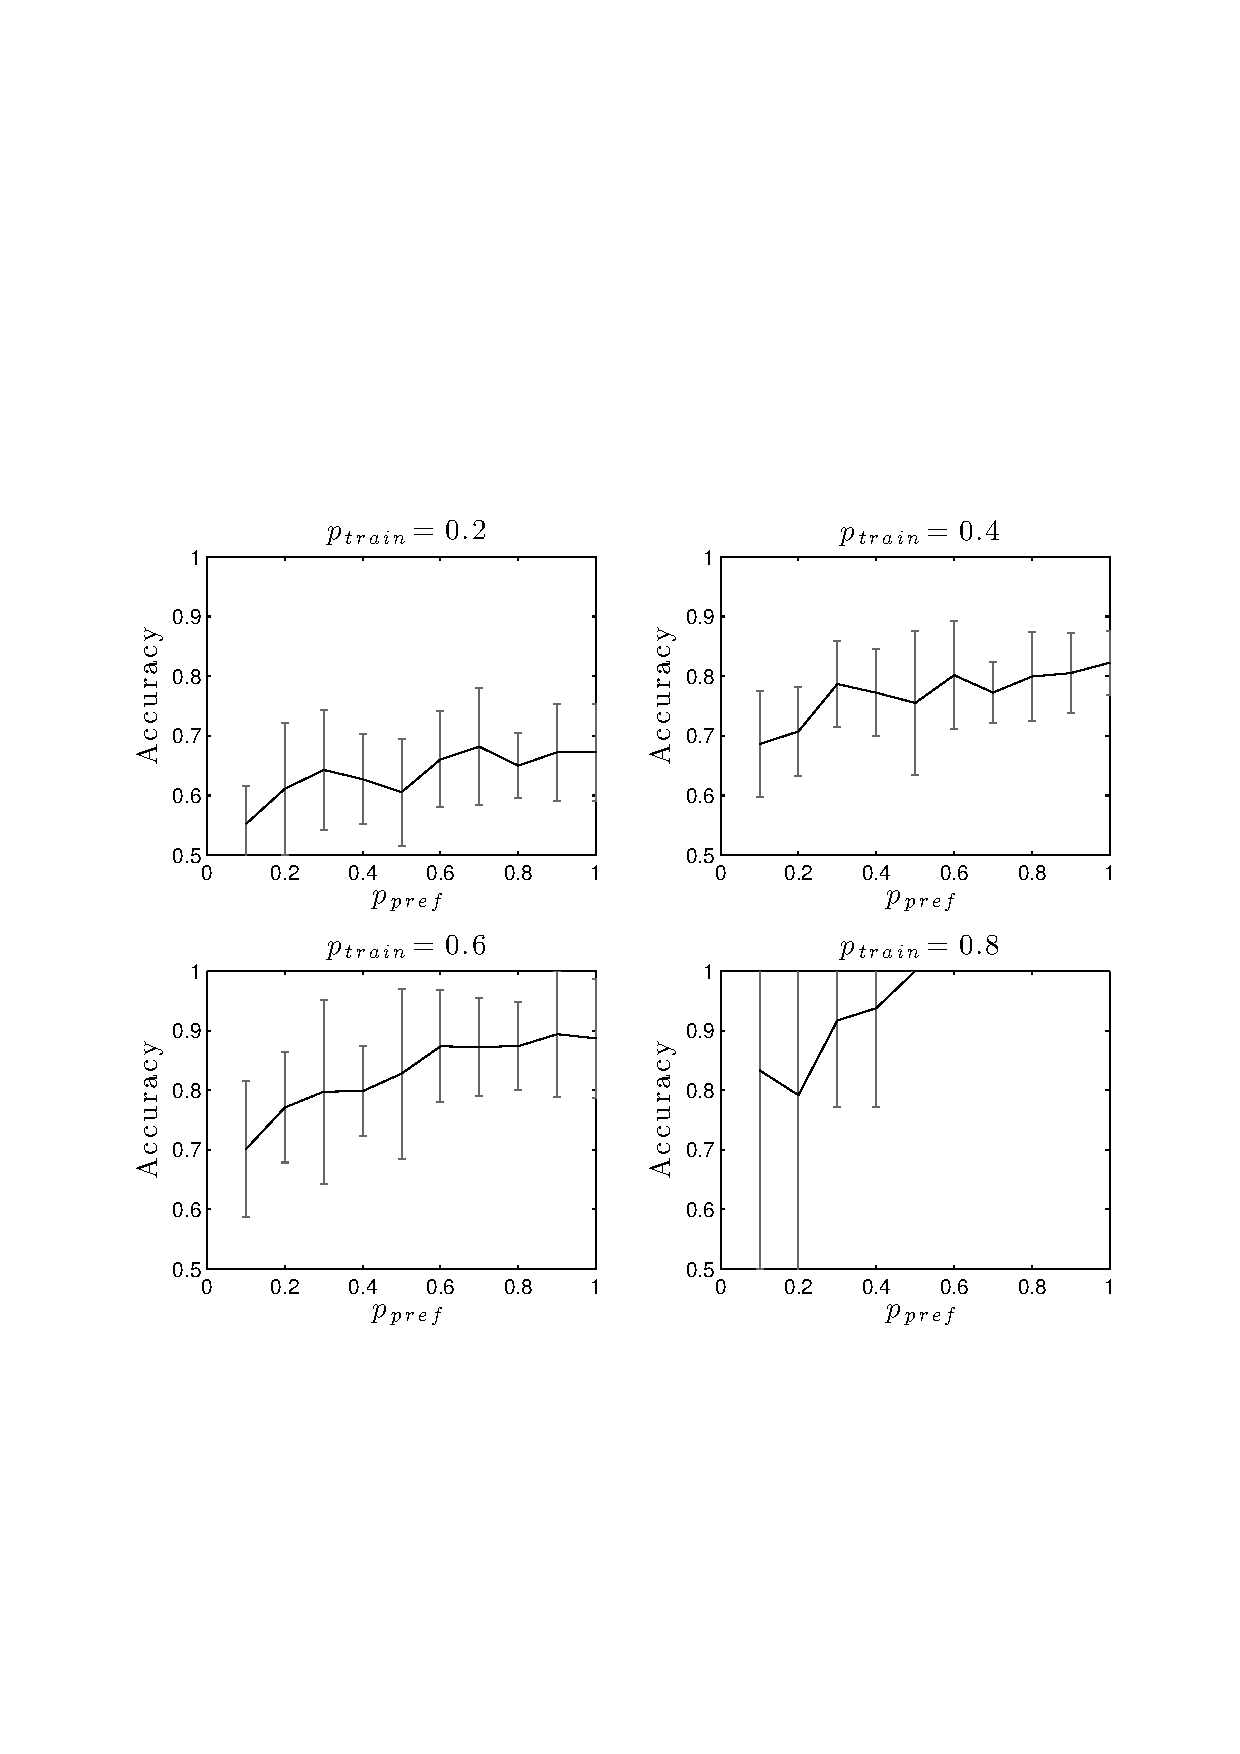
\includegraphics[width=1\linewidth]{accuracy.pdf}
  \caption{Influence of input size ($p_{train}$ and $p_{pref}$)}
  \label{fig:fractie}
\end{figure}

Figure~\ref{fig:fractie} shows how the accuracy improve as the fractions of examples ($p_{train}$) and preferences ($p_{pref}$) that are used for learning increase.
In all cases, more than half the pairs of examples are correctly predicted and the high accuracy values can be obtained even for small datasets.
Additional experiments have shown that even for lower accuracy values the learned optimization criteria are often capable of identifying the correct optimal solution \cite{kolb2015thesis}.

The standard underlying model can be directly expressed using the soft constraints that can be learned.
Even though clausal theories can be very expressive, important restrictions have been placed on the learned clauses in this paper.
In order to test the accuracy for models which cannot be directly expressed, a model consisting of two disconnected clauses has been tested as well.
While there are limits to the expressibility, the learned optimization criteria were able to obtain similar levels of accuracy and seem to be robust with respect to the exact formulation.

\begin{question}[Errors]
  What is the influence of errors in preferences on the accuracy?
\end{question}

The influence of errors is shown in Figure~\ref{fig:ruis}.
For this experiment, the second approach of testing has been applied, using overlapping training and test sets ($\sym{E}_{train} = \sym{E}_{test} = \sym{E}$).
High accuracy values are obtained, despite significant numbers of errors.
The figure also shows that increasing the number of preferences used for learning ($p_{pref}$) improves the robustness of the algorithm, even if the relative amount of errors ($p_{error}$) remains unchanged.

\begin{figure}
  \centering
    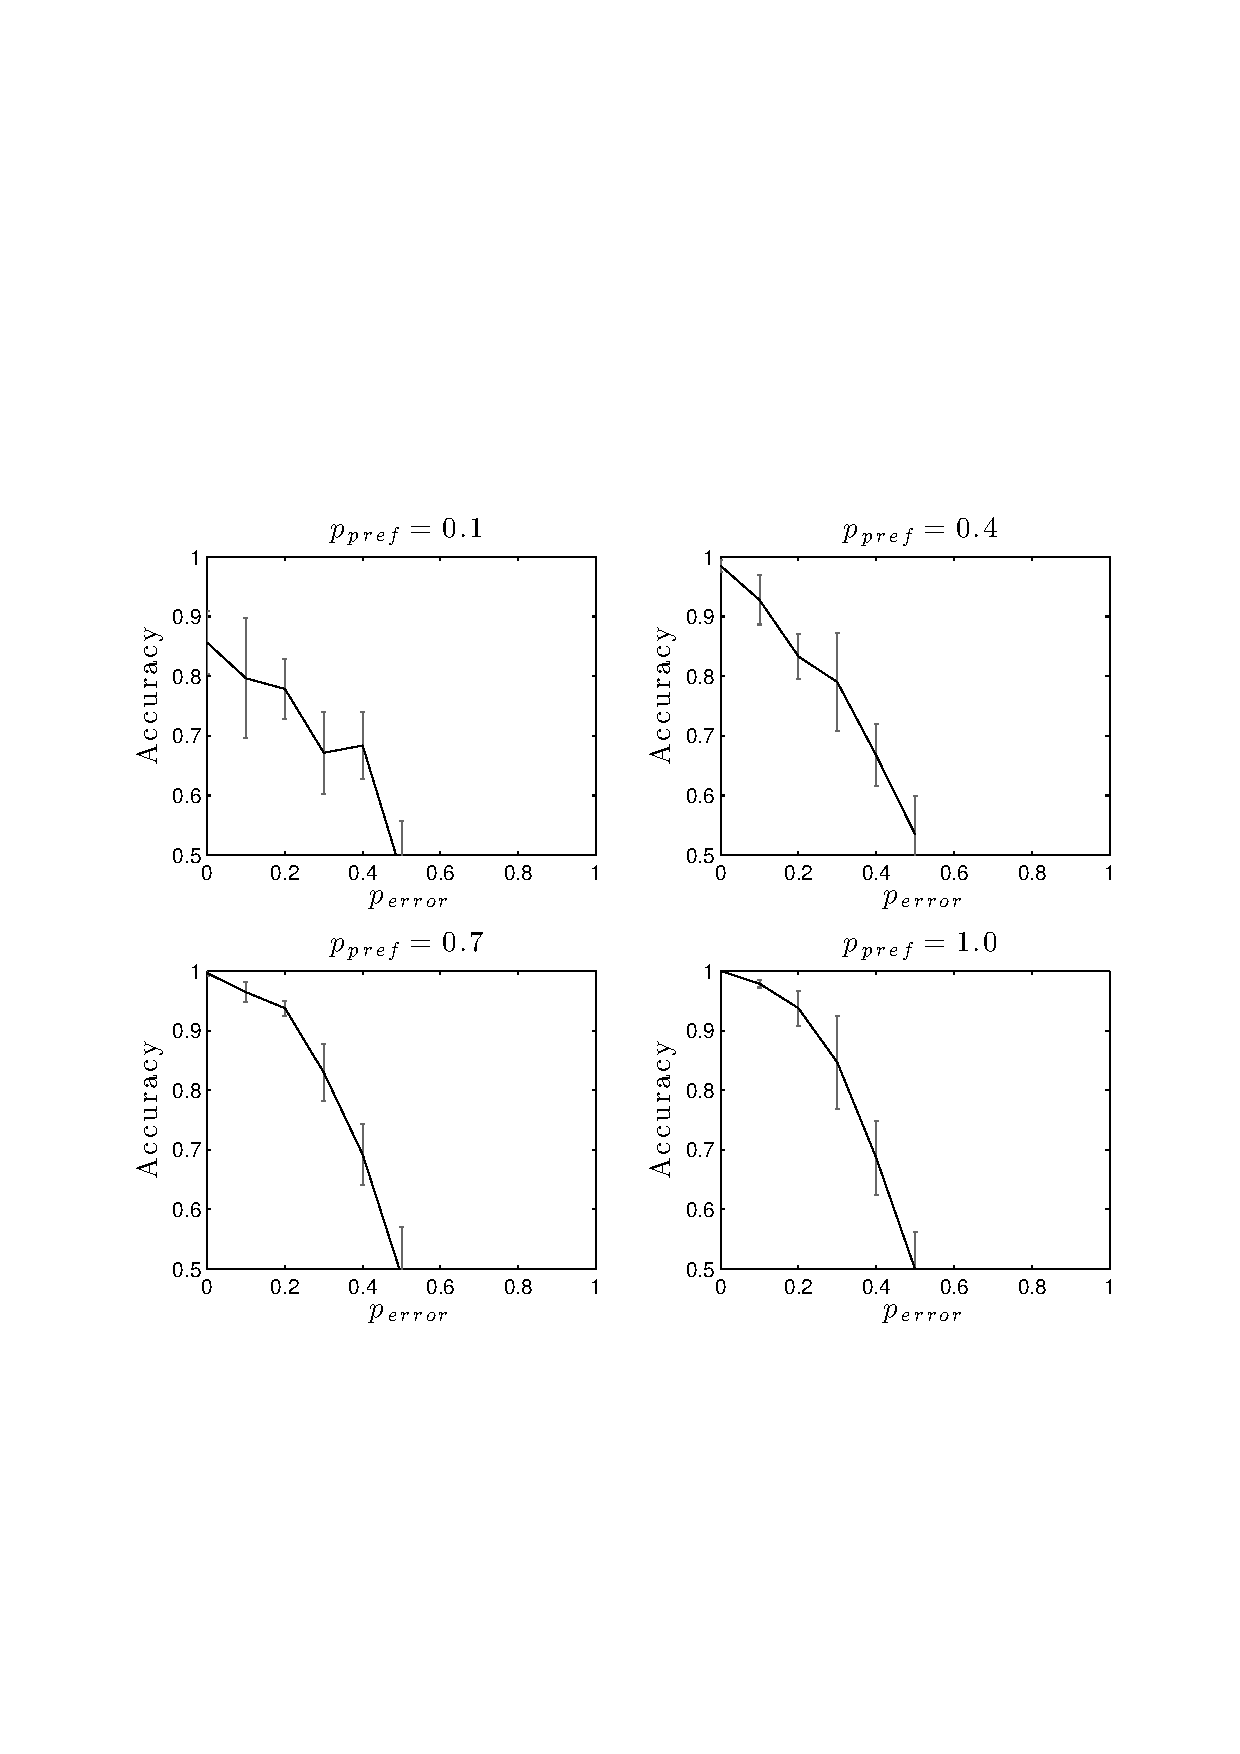
\includegraphics[width=1\linewidth]{errors.pdf}
  \caption{Influence of preference errors ($p_{error}$)}
  \label{fig:ruis}
\end{figure}

  \begin{table}[!htp]
    \caption{Accuracy for different thresholds ($t$)}
    \begin{tabularx}{\linewidth}{XXXX}
      $t = 1$ & $t = 2$ & $t = 3$ & $t = 4$ \\
      \toprule
     0.823 & 0.740 & 0.788 & 0.735 \\
     ($\pm$ 0.073) & ($\pm$ 0.078) & ($\pm$ 0.074) & ($\pm$ 0.063)
    \end{tabularx}
    \label{tbl:limiet}
  \end{table}

\begin{question}[Threshold]
  What is the effect of the soft constraint threshold on the accuracy?
\end{question}

Table~\ref{tbl:limiet} demonstrates that increasing the threshold used for finding soft constraints does not improve the accuracy ($p_{train} = p_{pref} = 0.4$).
However, if the number of examples is increased, a higher threshold will likely be appropriate.

% -------------------------------------------------
% Conclusion
% -------------------------------------------------

\section{Conclusion}
We presented an approach to automatically acquire constraints and optimization criteria from examples and preferences.
Implementations for both clause discovery and clausal optimization were provided that accomplish these tasks using first-order logic clauses.

The constraint learning implementation has been able to learn the relevant hard and soft constraints in all experiments.
For each problem, the relevant constraints could be learned from only a few examples.
Although the system requires only examples and preferences, users can provide more information through background knowledge.
The constraints learned by clausal discovery are independent of the constants of specific problem instantiations (examples), which facilitates the construction of positive examples.

Using the constraint learning implementation, the goal of learning a weighted first-order MAX-SAT model has been accomplished.
The learned models allow optimal solutions to be found.
Even for small datasets and erroneous preferences, optimization criteria are found that rank most examples correctly.

Aside from learning formal representations automatically from examples, we have shown how these representations can be used in practice.
This also forms an important step to enable the learning of optimization criteria in an interactive setting.

\paragraph{Future work}
There are several opportunities for future work.
In the current approach weight learning is performed using preferences and a learn-to-rank SVM.
It would, however, be easy to use another type of input (e.g. absolute scores) and a corresponding SVM.

It would be interesting to adapt the number of variables and literals per clause dynamically, as they have a strong influence on the efficiency and accuracy of the clause learning system.
Additionally, interactivity could be added to the learning system by actively generating examples or preferences and querying the user about their validity.

Finally, it would be desirable to improve the implementation in order to tackle larger sized problems.
All the experiments were conducted with problems of limited size and the computation time increases rapidly if there are more predicates, variables and literals to be used in clauses.

\section*{Acknowledgments}
The author thanks his promoters Luc De Raedt and Anton Dries.
Furthermore, he is is thankful for the help provided by Bart Bogaerts, Jesse Davis, Marc Denecker, Vladimir Dzyuba, Angelika Kimmig and Jan Tobias M\"uhlberg.
Samuel Kolb is supported by the Research Foundation - Flanders (FWO).

% -------------------------------------------------
% Bibliography
% -------------------------------------------------

\begin{thebibliography}{}

\bibitem[\protect\citeauthoryear{Beldiceanu and
  Simonis}{2012}]{Beldiceanu:ModelSeeker}
Beldiceanu, N., and Simonis, H.
\newblock 2012.
\newblock A model seeker: Extracting global constraint models from positive
  examples.
\newblock In {\em Principles and Practice of Constraint Programming},
  141--157.
\newblock Springer.

\bibitem[\protect\citeauthoryear{Bessiere \bgroup et al\mbox.\egroup
  }{2007}]{bessiere2007query}
Bessiere, C.; Coletta, R.; O'Sullivan, B.; Paulin, M.; et~al.
\newblock 2007.
\newblock Query-driven constraint acquisition.
\newblock In {\em Proceedings of the Twentieth International Joint Conference
  on Artificial Intelligence},  50--55.

\bibitem[\protect\citeauthoryear{Bessiere \bgroup et al\mbox.\egroup
  }{2013}]{bessiere2013constraint}
Bessiere, C.; Coletta, R.; Hebrard, E.; Katsirelos, G.; Lazaar, N.; Narodytska,
  N.; Quimper, C.-G.; and Walsh, T.
\newblock 2013.
\newblock Constraint acquisition via partial queries.
\newblock In {\em Proceedings of the Twenty-Third International Joint
  Conference on Artificial Intelligence},  475--481.
\newblock AAAI Press.

\bibitem[\protect\citeauthoryear{Campigotto, Passerini, and
  Battiti}{2011}]{campigotto2011active}
Campigotto, P.; Passerini, A.; and Battiti, R.
\newblock 2011.
\newblock Active learning of combinatorial features for interactive
  optimization.
\newblock In {\em Learning and Intelligent Optimization}. Springer.
\newblock  336--350.

\bibitem[\protect\citeauthoryear{De~Pooter, Wittocx, and
  Denecker}{2013}]{de2013prototype}
De~Pooter, S.; Wittocx, J.; and Denecker, M.
\newblock 2013.
\newblock A prototype of a knowledge-based programming environment.
\newblock In {\em Applications of Declarative Programming and Knowledge
  Management}. Springer.
\newblock  279--286.

\bibitem[\protect\citeauthoryear{De~Raedt and
  Dehaspe}{1997}]{DeRaedt:ClausalDiscovery}
De~Raedt, L., and Dehaspe, L.
\newblock 1997.
\newblock Clausal discovery.
\newblock {\em Machine Learning} 26(2-3):99--146.

\bibitem[\protect\citeauthoryear{Joachims}{2006}]{joachims2006training}
Joachims, T.
\newblock 2006.
\newblock Training linear svms in linear time.
\newblock In {\em Proceedings of the 12th ACM SIGKDD international conference
  on Knowledge discovery and data mining},  217--226.
\newblock ACM.

\bibitem[\protect\citeauthoryear{Kok and Domingos}{2005}]{kok2005learning}
Kok, S., and Domingos, P.
\newblock 2005.
\newblock Learning the structure of markov logic networks.
\newblock In {\em Proceedings of the 22nd international conference on Machine
  learning},  441--448.
\newblock ACM.

\bibitem[\protect\citeauthoryear{Kolb}{2015}]{kolb2015thesis}
Kolb, S.
\newblock 2015.
\newblock Learning constraints and optimization criteria.
\newblock Master's thesis, KULeuven.

\bibitem[\protect\citeauthoryear{Lallouet \bgroup et al\mbox.\egroup
  }{2010}]{Lallouet:LearningCP}
Lallouet, A.; Lopez, M.; Martin, L.; and Vrain, C.
\newblock 2010.
\newblock On learning constraint problems.
\newblock In {\em Tools with Artificial Intelligence (ICTAI), 2010 22nd IEEE
  International Conference on}, volume~1,  45--52.
\newblock IEEE.

\bibitem[\protect\citeauthoryear{Metzler and Croft}{2007}]{metzler2007linear}
Metzler, D., and Croft, W.~B.
\newblock 2007.
\newblock Linear feature-based models for information retrieval.
\newblock {\em Information Retrieval} 10(3):257--274.

\bibitem[\protect\citeauthoryear{Puget}{2004}]{Wallace:PrinciplesCP}
Puget, J.-F.
\newblock 2004.
\newblock Constraint programming next challenge: Simplicity of use.
\newblock In Wallace, M., ed., {\em Principles and Practice of Constraint
  Programming - CP 2004}, volume 3258 of {\em Lecture Notes in Computer
  Science}. Springer Berlin Heidelberg.
\newblock  5--8.

\bibitem[\protect\citeauthoryear{Wittocx, Mari{\"e}n, and
  Denecker}{2008}]{wittocx2008idp}
Wittocx, J.; Mari{\"e}n, M.; and Denecker, M.
\newblock 2008.
\newblock The idp system: a model expansion system for an extension of
  classical logic.
\newblock In {\em Proceedings of the 2nd Workshop on Logic and Search},
  153--165.

\end{thebibliography}
\bibliographystyle{aaai}
\end{document}
